\section{Fine-tuning Method: Multi-context Self-Distillation}
\label{sec:finetuning}

PrismMathQA's runtime framework can improve answer grounding and verification, but it cannot by itself make the base model a better mathematical reasoner. The model still needs training signals that reward correct reasoning trajectories and discourage misleading intermediate steps. This section presents Adaptive-View Self-Distillation (AVSD) \citep{nguyen2026avsd} as the finetuning method for the model used by PrismMathQA. For this report, the finetuning data is a MetaMathQA subset whose examples provide a problem statement and solution artifacts. The method is especially well matched to a math tutor because these examples naturally come with multiple contexts: a full reference solution, a partial rationale, a final answer, and a concise hint. These contexts are useful during training but are not all available to the student model at inference time.

Knowledge distillation is a standard way to transfer behavior from a teacher model or teacher distribution into a smaller or task-specialized student model \citep{hinton2015distilling}. In language-model post-training, distillation is attractive because it provides richer supervision than a single binary correctness label: the student can learn from token probabilities, solution traces, or preferred reasoning styles. For mathematical reasoning, this is especially useful because many errors are local. A final answer may be wrong because of one algebraic step, one sign error, or one invalid simplification; dense distillation can in principle teach the model which intermediate tokens should become more or less likely.

However, the classical teacher-student setup is not automatically effective for reasoning. If the teacher trajectory is offline and fixed, the student may be trained on states that it will not visit at inference time. If the teacher has privileged information, such as a full solution, the student may imitate tokens that depend on information unavailable in the real prompt. If a single teacher view is chosen, the training signal can inherit that view's bias: a full solution may over-constrain the reasoning path, while a final answer may be too sparse to guide intermediate steps. AVSD addresses these limitations by keeping training on-policy and by aggregating multiple privileged views rather than trusting one teacher context.

\begin{figure}[t]
\centering
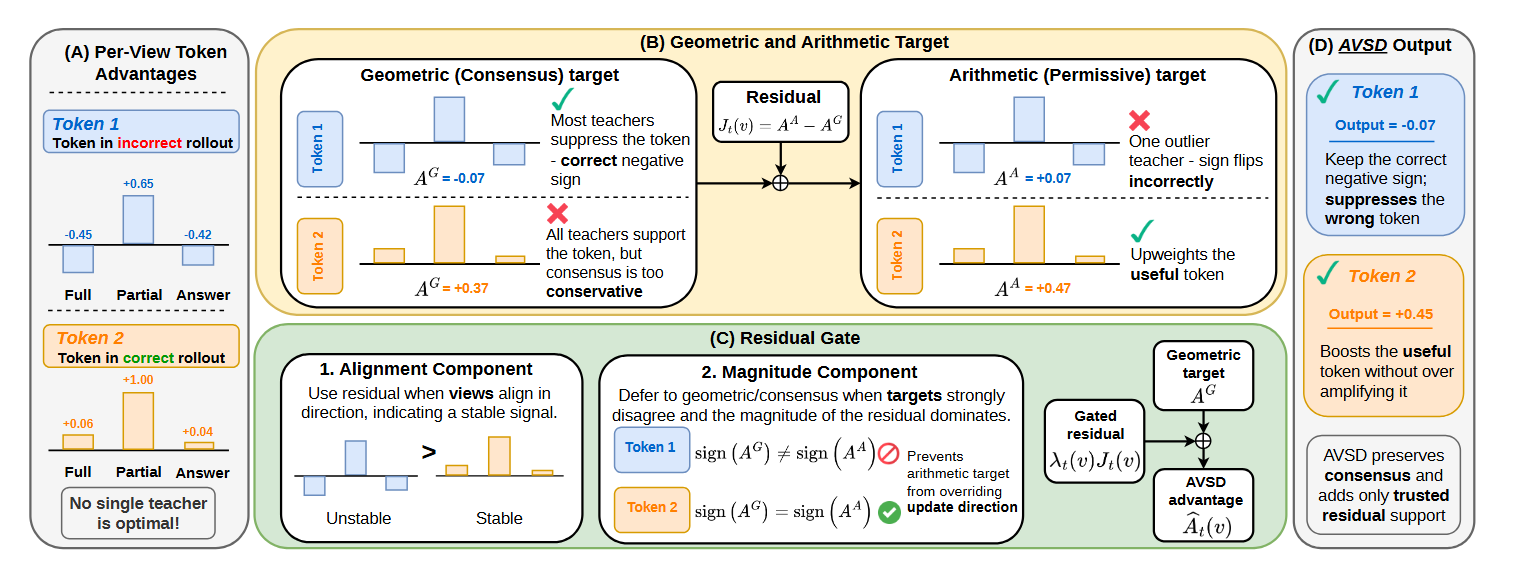
\includegraphics[width=0.95\linewidth]{imgs/avsd_pipeline.png}
\caption{AVSD training pipeline used as the finetuning method for PrismMathQA. The student generates on-policy rollouts from the problem statement, while multiple privileged teacher views provide token-level supervision. AVSD separates cross-view consensus from view-specific residual signals and gates the residual before constructing the final distillation target.}
\label{fig:avsd-pipeline}
\end{figure}

Figure~\ref{fig:avsd-pipeline} summarizes the training flow. The student sees only the math problem and produces a rollout. The teacher mode evaluates the same rollout under four privileged contexts: full solution, partial rationale, final answer, and concise hint. The algorithm then combines these teacher distributions into a reconstructed target that preserves stable agreement while filtering view-specific signals that may be unreliable.

\subsection{From Single-view Self-Distillation to Token Advantages}

Let $D$ be a training set of examples $(x,r)$, where $x$ is the student-visible prompt and $r$ is privileged training-time information. In a math setting, $x$ can be the problem statement and $r$ can be a reference solution or answer annotation. The student model observes only $x$ during rollout and samples
\[
    y = (y_1,\ldots,y_T) \sim P_{\theta}^{S}(\cdot \mid x).
\]
At position $t$, define the prefix
\[
    h_t = (x, y_{<t})
\]
and the student next-token distribution
\[
    p_t(v) := P_{\theta}^{S}(Y_t=v \mid h_t), \qquad v \in \mathcal{V},
\]
where $\mathcal{V}$ is the vocabulary.

In standard single-view self-distillation, the same model is evaluated again in a teacher mode that receives privileged context $r$. At the same prefix $h_t$, the teacher distribution is
\[
    q_t(v) := \operatorname{sg}\left[P_{\theta}^{T}(Y_t=v \mid h_t,r)\right],
\]
where $\operatorname{sg}[\cdot]$ denotes stop-gradient. The teacher is not a separate larger model; it is the same model under richer conditioning. The local reverse-KL distillation term is
\[
    \ell_t(\theta)=D_{\mathrm{KL}}(p_t \Vert q_t)
    = \sum_{v\in\mathcal{V}} p_t(v)\left(\log p_t(v)-\log q_t(v)\right).
\]
Using $\nabla_\theta p_t(v)=p_t(v)\nabla_\theta\log p_t(v)$, its gradient can be written as
\[
\begin{aligned}
    \nabla_\theta \ell_t
    &= \sum_{v\in\mathcal{V}} \nabla_\theta p_t(v)
       \left(\log p_t(v)-\log q_t(v)+1\right)\\
    &= \mathbb{E}_{v\sim p_t}
       \left[\left(\log p_t(v)-\log q_t(v)+1\right)
       \nabla_\theta\log p_t(v)\right].
\end{aligned}
\]
The constant $1$ is a baseline because
\[
    \mathbb{E}_{v\sim p_t}[\nabla_\theta\log p_t(v)] = 0.
\]
Therefore,
\[
    \nabla_\theta \ell_t
    = \mathbb{E}_{v\sim p_t}
       \left[\left(\log p_t(v)-\log q_t(v)\right)
       \nabla_\theta\log p_t(v)\right].
\]
Gradient descent on $\ell_t$ moves in the direction
\[
    \mathbb{E}_{v\sim p_t}\left[A_t(v)\nabla_\theta\log p_t(v)\right],
\]
where
\[
    A_t(v) := \log q_t(v)-\log p_t(v).
    \label{eq:single-advantage}
\]
This is the token-level distillation advantage. If $A_t(v)>0$, the teacher assigns token $v$ higher probability than the student, so training promotes that token. If $A_t(v)<0$, training suppresses it. The intuition is close to policy-gradient reinforcement learning, but the reward is a dense teacher-student probability comparison at every token rather than a sparse final-answer reward.

For PrismMathQA, this is important because many wrong math answers contain both useful and harmful tokens. A sparse verifier might only say that the final answer is incorrect. The reverse-KL advantage can instead identify which generated tokens the privileged teacher would have made more or less likely at each prefix. This dense feedback is valuable for learning step-by-step reasoning.

\subsection{Multi-view Privileged Contexts}

Single-view self-distillation requires choosing one privileged context. In mathematics, that choice is unstable. A full reference solution gives detailed supervision but may overfit to one derivation. A partial rationale can provide useful early structure while leaving room for the student model to complete the solution. A final answer is compact and avoids forcing a chain of thought, but it gives weak local guidance. A concise hint points to the key theorem, substitution, or transformation without revealing the full derivation. AVSD treats these four contexts as a teacher family rather than selecting one.

Let the training example contain privileged information $r$, and let
\[
    \mathcal{V}(r)=\{r^{(1)},\ldots,r^{(M)}\}
\]
be $M$ transformed views, where $r^{(m)}=T_m(r)$. For PrismMathQA math finetuning, the default setting uses four views:
\[
\begin{aligned}
    r^{(1)}&=\text{full solution}, &
    r^{(2)}&=\text{partial rationale},\\
    r^{(3)}&=\text{final answer}, &
    r^{(4)}&=\text{concise hint}.
\end{aligned}
\]
Each view induces a teacher distribution at the same student prefix:
\[
    q_t^{(m)}(v)
    := \operatorname{sg}\left[P_{\theta}^{T}(Y_t=v\mid h_t,r^{(m)})\right],
    \qquad m=1,\ldots,M.
\]
The per-view token advantage is
\[
    \Delta_t^{(m)}(v)
    := \log q_t^{(m)}(v)-\log p_t(v).
\]
The central problem is how to combine these advantages. Averaging all teachers too permissively can allow one view to dominate. Requiring all teachers to agree can be too conservative and can discard useful view-specific information. AVSD solves this by decomposing the multi-view signal into consensus and residual components.

\begin{table}[t]
\centering
\caption{Math privileged views used by AVSD-style PrismMathQA training.}
\label{tab:math-views}
\small
\begin{tabular}{p{0.21\linewidth}p{0.34\linewidth}p{0.34\linewidth}}
\toprule
View & Teacher context & Training role \\
\midrule
Full solution & Complete worked derivation with final answer. & Provides dense reasoning supervision and exposes the full mathematical structure of the solution. \\
\midrule
Partial rationale & Initial reasoning steps or a truncated rationale. & Guides the model toward a useful start without forcing every later step to match a reference trace. \\
\midrule
Final answer & Gold answer without full derivation. & Supplies compact correctness information while allowing the model to search for its own explanation path. \\
\midrule
Concise hint & Short mathematical hint such as the key substitution, theorem, or transformation. & Encourages the model to discover the missing derivation while still pointing it toward a productive strategy. \\
\bottomrule
\end{tabular}
\end{table}

Table~\ref{tab:math-views} defines the four math-specific privileged contexts used in PrismMathQA. The concise-hint view is included as a first-class view because it matches tutoring behavior: it reveals a useful strategy without exposing a complete solution. In the equations below, $M=4$ for the default PrismMathQA setup, although the same AVSD objective can be ablated with fewer views in Section~4.

\subsection{Geometric Consensus Target}

The geometric target captures intersection support across teacher views. Define the unnormalized geometric score
\[
    \widetilde{q}_t^G(v)
    := \left(\prod_{m=1}^{M}q_t^{(m)}(v)\right)^{1/M}
    = \exp\left(\frac{1}{M}\sum_{m=1}^{M}\log q_t^{(m)}(v)\right),
\]
and normalize it as
\[
    q_t^G(v)
    := \frac{\widetilde{q}_t^G(v)}
    {\sum_{u\in\mathcal{V}}\widetilde{q}_t^G(u)}.
\]
The geometric mean is conservative. A token receives high support only if it is supported across views. If the full-solution teacher strongly promotes a token but the partial-rationale and answer-only teachers suppress it, the geometric score decreases. This is desirable when the token depends on details that only one privileged view reveals.

For advantage analysis, AVSD uses the unnormalized geometric score because normalization contributes only a token-independent constant. The geometric advantage is
\[
\begin{aligned}
    A_t^G(v)
    &:= \log \widetilde{q}_t^G(v)-\log p_t(v)\\
    &= \frac{1}{M}\sum_{m=1}^{M}\log q_t^{(m)}(v)-\log p_t(v)\\
    &= \frac{1}{M}\sum_{m=1}^{M}
       \left(\log q_t^{(m)}(v)-\log p_t(v)\right)\\
    &= \frac{1}{M}\sum_{m=1}^{M}\Delta_t^{(m)}(v).
\end{aligned}
\]
Thus the consensus advantage is the average signed update induced by the teacher family. If most views agree that a token should be suppressed, $A_t^G(v)$ is negative. If they agree it should be promoted, $A_t^G(v)$ is positive. For a tutor model, this consensus is the safest part of the training signal because it is less likely to depend on a single privileged annotation format.

\subsection{Arithmetic Marginal Target}

The arithmetic target captures union support. It is defined as
\[
    q_t^A(v) := \frac{1}{M}\sum_{m=1}^{M}q_t^{(m)}(v),
\]
with arithmetic advantage
\[
    A_t^A(v) := \log q_t^A(v)-\log p_t(v).
\]
This target is permissive: a token can receive high probability if any view strongly supports it. Such support can be useful. For example, an answer-only view may make a concise algebraic transition more likely, while a full-solution view may favor a detailed explanatory phrase. A good tutor should be able to learn from both signals.

The weakness of the arithmetic target is that it can preserve artifacts. A token may be strongly supported because one privileged view exposes information that the student model cannot infer from the prefix. Directly distilling from $q_t^A$ can therefore encourage tokens whose support is not robust under the student-visible context. In educational terms, the model may learn to imitate a teacher that has already seen the solution rather than learn a reasoning step that follows from the problem.

\subsection{Cross-view Residual}

The gap between the arithmetic and geometric targets isolates view-specific support. AVSD defines the residual
\[
    J_t(v) := \log q_t^A(v)-\log \widetilde{q}_t^G(v).
\]
By the arithmetic-geometric mean inequality, $q_t^A(v)\geq \widetilde{q}_t^G(v)$, so
\[
    J_t(v)\geq 0.
\]
The arithmetic advantage can be decomposed as
\[
    A_t^A(v)=A_t^G(v)+J_t(v).
\]
This equation is the key decomposition. $A_t^G(v)$ is the shared signal: it says what the teacher family agrees about. $J_t(v)$ is the additional support retained by the permissive target but absent from strict consensus. A small residual means the views agree. A large residual means at least one view assigns much more support than the others.

The residual is not automatically good or bad. It may contain complementary evidence that improves the model, or it may contain privileged leakage. AVSD therefore does not discard it, but also does not trust it unconditionally. The method keeps the consensus direction and gates the residual contribution.

\subsection{Residual Gate}

AVSD reconstructs a token-level advantage
\[
    \widehat{A}_t(v)
    := A_t^G(v)+\lambda_t(v)J_t(v),
    \qquad \lambda_t(v)\in[0,1].
\]
The gate $\lambda_t(v)$ has two components: an alignment component and a magnitude component.

The alignment component checks whether the per-view advantages agree in sign. It is defined as
\[
    C_t(v)
    :=
    \frac{|A_t^G(v)|}
    {\frac{1}{M}\sum_{m=1}^{M}|\Delta_t^{(m)}(v)|+\epsilon}
    =
    \frac{
    \left|\frac{1}{M}\sum_{m=1}^{M}\Delta_t^{(m)}(v)\right|}
    {\frac{1}{M}\sum_{m=1}^{M}|\Delta_t^{(m)}(v)|+\epsilon}.
\]
If the teacher views point in the same direction, the numerator is close to the denominator and $C_t(v)$ is high. If some views promote a token while others suppress it, the signed average can cancel and $C_t(v)$ is low. This distinguishes useful complementary support from direct conflict.

The magnitude component checks whether the residual is proportionate to the consensus:
\[
    R_t(v)
    :=
    \frac{|A_t^G(v)|}{|A_t^G(v)|+J_t(v)+\epsilon}.
\]
If the residual is much larger than the consensus, then the arithmetic target may override the direction established by the teacher family. In that case $R_t(v)$ becomes small. If the residual is moderate relative to the consensus, $R_t(v)$ allows the residual to adjust the update magnitude.

The final gate is
\[
    \lambda_t(v)
    =
    C_t(v)R_t(v)
    =
    C_t(v)
    \frac{|A_t^G(v)|}{|A_t^G(v)|+J_t(v)+\epsilon}.
    \label{eq:avsd-gate}
\]
This gate acts as an adaptive regularizer. It admits view-specific information when the views agree on direction and when the residual is not too large. It suppresses residual information when the views conflict, when consensus is weak, or when one view tries to dominate.

The boundedness property follows directly:
\[
    \lambda_t(v)J_t(v)
    =
    C_t(v)\frac{|A_t^G(v)|J_t(v)}
    {|A_t^G(v)|+J_t(v)+\epsilon}
    \leq |A_t^G(v)|.
\]
Since $C_t(v)\leq 1$ and the denominator is at least $J_t(v)$, the gated residual cannot exceed the consensus magnitude. Therefore, if $A_t^G(v)<0$, the reconstructed advantage cannot be flipped to a large positive value solely by a residual from one privileged view. This is the protection against privileged-view leakage: residual support can strengthen a trusted direction, but it cannot freely reverse it.

\subsection{Reconstructed Target and AVSD Loss}

The reconstructed target corresponding to $\widehat{A}_t$ is obtained by reweighting the geometric target with the gated residual and normalizing:
\[
    q_t^{\star}(v)
    =
    \frac{\widetilde{q}_t^G(v)\exp(\lambda_t(v)J_t(v))}
    {\sum_{u\in\mathcal{V}}\widetilde{q}_t^G(u)\exp(\lambda_t(u)J_t(u))}.
\]
This target blends token-level signals. If $\lambda_t(v)=0$, the token follows the geometric consensus target. If $\lambda_t(v)=1$ for all tokens, the method recovers the arithmetic marginal target. In practice, most tokens remain anchored to consensus, and only selected tokens receive residual support.

The final training objective is on-policy reverse-KL distillation to the reconstructed target:
\[
    \mathcal{L}_{\mathrm{AVSD}}(\theta)
    =
    \mathbb{E}_{(x,r)\sim D}
    \mathbb{E}_{y\sim P_{\theta}^{S}(\cdot\mid x)}
    \left[
    \sum_{t=1}^{|y|}
    D_{\mathrm{KL}}\left(
    p_{\theta}(\cdot\mid h_t)
    \Vert
    \operatorname{sg}[q_t^{\star}(\cdot)]
    \right)
    \right].
    \label{eq:avsd-loss}
\]
Gradients flow through the student distribution only. The teacher views and reconstructed targets are treated as fixed supervision at the current prefix. Equivalently, the sampled-token update uses the reconstructed advantage
\[
    \widehat{A}_t(y_t)=A_t^G(y_t)+\lambda_t(y_t)J_t(y_t).
\]

\subsection{Training Procedure for PrismMathQA}

In a PrismMathQA finetuning pipeline, each training iteration would proceed as follows. First, sample a math problem and its available privileged artifacts from the MetaMathQA subset. Second, generate an on-policy rollout from the current student model using only the problem statement. Third, construct the four privileged views: full solution, partial rationale, final answer, and concise hint. Fourth, evaluate the same model in teacher mode under each privileged view at the student-generated prefixes. Fifth, compute $A_t^G$, $q_t^A$, $J_t$, $\lambda_t$, $q_t^{\star}$, and the reverse-KL loss. Finally, update the model parameters by minimizing $\mathcal{L}_{\mathrm{AVSD}}$.

The computational overhead is controlled because all teacher views share the same student rollout. The expensive sequential generation path is not repeated for every view; the additional work is view-conditioned forward evaluation at existing prefixes. The AVSD paper reports a modest runtime increase from $41.5$ seconds per step for single-view OPSD to $46.7$ seconds per step for AVSD under the same Qwen3-4B setup \citep{nguyen2026avsd}. For PrismMathQA, this makes AVSD a plausible training extension rather than an entirely different serving architecture.

The method also matches the runtime philosophy. RAG, memory, and tools each add context to the tutor, but the system controls how that context enters the answer. AVSD applies the same idea during training: privileged contexts are useful, but they must be balanced so that the student learns reasoning behavior available at inference time. The result is a model that can be deployed inside the PrismMathQA agentic loop with stronger mathematical reasoning before retrieval and tool use are applied.
